\documentclass[aspectratio=141,10pt]{beamer}

% ---------- Look copied from the lecture slides: white, dark red titles, grey text ----------
\usepackage[T1]{fontenc}
\usepackage[scaled=0.92]{helvet}
\renewcommand{\familydefault}{\sfdefault}
\usepackage{amsmath,amssymb}
\usepackage{booktabs,tabularx,colortbl,array}
\usepackage{graphicx}
\usepackage{tikz}

\definecolor{aimsred}{HTML}{990000}
\definecolor{rowpink}{HTML}{F7E9E9}
\definecolor{textgrey}{HTML}{404040}

\usetheme{default}
\setbeamertemplate{navigation symbols}{}
\setbeamercolor{normal text}{fg=textgrey,bg=white}
\setbeamercolor{structure}{fg=aimsred}
\setbeamercolor{frametitle}{fg=aimsred,bg=white}
\setbeamerfont{frametitle}{series=\bfseries,size=\LARGE}
\setbeamertemplate{frametitle}{\vskip1.2em\centering\usebeamerfont{frametitle}\usebeamercolor[fg]{frametitle}\insertframetitle\par\vskip0.4em}
\setbeamertemplate{itemize item}{\color{aimsred}$\bullet$}
\setbeamertemplate{itemize subitem}{\color{aimsred}$\circ$}
\setbeamertemplate{footline}{\hfill\color{textgrey}\footnotesize\insertframenumber\hspace{1em}\vspace{0.6em}}

% Rounded red callout box, like the "Assumption" box in the lectures
\newcommand{\callout}[2]{%
  \begin{center}\fcolorbox{aimsred}{rowpink!60}{\begin{minipage}{#1}\centering #2\end{minipage}}\end{center}}
\newcommand{\hl}[1]{{\bfseries\color{aimsred}#1}}

\title{Comparing stochastic and deterministic models of an endemic infection}
\subtitle{Project 3, Part 1: the SIRS model}
\author{}
\date{}

\begin{document}

% ---------------- Title ----------------
\begin{frame}[plain]
\centering
\vspace{0.5em}

\includegraphics[height=2.4cm]{img/logo1.png}\\[1.6em]
{\Large\color{textgrey} Training Workshop on Mathematical Biology 2026}\\[1.2em]
{\Large\bfseries\color{aimsred} Project 3: stochastic versus deterministic models\\[0.3em]
Part 1: SIRS endemic equilibrium\\ Part 2: two strains with waning immunity}\\[2.2em]

\includegraphics[height=1.3cm]{img/logo2.png}\hspace{1.5cm}

\includegraphics[height=1.0cm]{img/logo3.png}\hspace{1.5cm}

\includegraphics[height=0.9cm]{img/logo0.png}
\end{frame}

% ---------------- Question ----------------
\begin{frame}{What we want to know}
\begin{itemize}\setlength\itemsep{0.7em}
  \item Start from the SIR model of Monday and Tuesday.
  \item Let recovered people lose their immunity and become susceptible again.
  \item Model the same system in two ways: an ODE model and an event based stochastic model (Gillespie SSA).
  \item Ask when the infection settles at an \hl{endemic} level, and whether the two models agree.
\end{itemize}
\callout{0.8\textwidth}{\textbf{Main question:} if the ODE says the disease persists, does the stochastic model say the same?}
\end{frame}

% ---------------- Cartoon ----------------
\begin{frame}{Q1. The model as a cartoon}
\centering
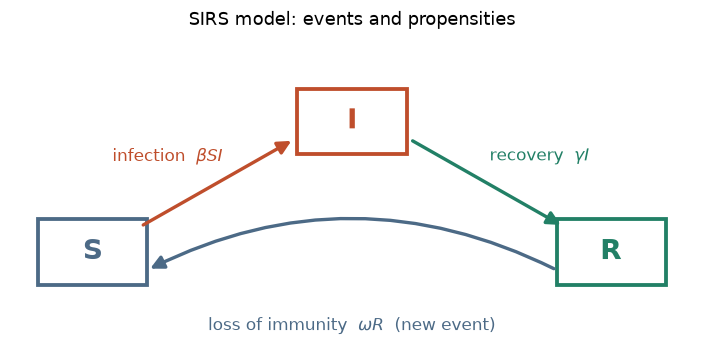
\includegraphics[width=0.78\textwidth]{img/fig1.png}\\[0.4em]
\begin{itemize}
  \item State $\mathbf x=[S,I,R]$ with $N=S+I+R$ fixed (no births or deaths).
  \item The new arrow is $R\to S$. It closes the loop $S\to I\to R\to S$.
\end{itemize}
\end{frame}

% ---------------- Events table ----------------
\begin{frame}{Q1 and Q2. Events, state change vectors, propensities}
\renewcommand{\arraystretch}{1.5}
\centering
\begin{tabular}{>{\columncolor{white}}l c c c}
\rowcolor{aimsred}\color{white}\bfseries Event & \color{white}\bfseries Reaction & \color{white}\bfseries Vector $[\Delta S,\Delta I,\Delta R]$ & \color{white}\bfseries Propensity $a_j(\mathbf x)$\\
Infection & $S+I\to 2I$ & $[-1,+1,\;0]$ & $\beta\,S\,I$\\
\rowcolor{rowpink} Recovery & $I\to R$ & $[\;0,-1,+1]$ & $\gamma\,I$\\
Loss of immunity & $R\to S$ & $[+1,\;0,-1]$ & $\omega\,R$\\
\end{tabular}
\vspace{1em}
\begin{itemize}\setlength\itemsep{0.5em}
  \item Loss of immunity is a first order event, like cell death on the propensity slide of the CME lecture ($X_i\to$ products, $a=k\,x_i$).
  \item Each of the $R$ people loses immunity at rate $\omega$, so $a_3=\omega R$. The mean immune time is $1/\omega$.
  \item Infection uses the mass action form $k\,x_ix_j$ from the same slide, so no division by $N$.
\end{itemize}
\end{frame}

% ---------------- ODE ----------------
\begin{frame}{Q3. The ODE model}
\[
\frac{dS}{dt}=-\beta SI+\omega R,\qquad
\frac{dI}{dt}=\beta SI-\gamma I,\qquad
\frac{dR}{dt}=\gamma I-\omega R
\]
\begin{itemize}\setlength\itemsep{0.6em}
  \item Each event adds its propensity times its state change vector.
  \item The three equations add up to zero, so $S+I+R=N$ stays constant.
  \item Equilibria: set every derivative to zero.
\end{itemize}
\callout{0.85\textwidth}{From $dR/dt=0$: $R^*=\dfrac{\gamma}{\omega}I^*$. \quad From $dI/dt=0$: $I^*(\beta S^*-\gamma)=0$.}
\end{frame}

% ---------------- Equilibria ----------------
\begin{frame}{Q3. Two equilibria and a critical population size}
\begin{columns}[T]
\column{0.47\textwidth}
\textbf{\color{aimsred} Disease free}\\[0.3em]
$I^*=0,\; R^*=0,\; S^*=N$\\[0.3em]
It always exists.\\[1.2em]
\textbf{\color{aimsred} Endemic}\\[0.3em]
$S^*=\dfrac{\gamma}{\beta}$, and from $N=S^*+I^*+R^*$:
\[ N=\frac{\gamma}{\beta}+I^*\Big(1+\frac{\gamma}{\omega}\Big)\]
\column{0.5\textwidth}
\callout{0.95\columnwidth}{%
$\displaystyle I^*=\frac{\omega}{\omega+\gamma}\Big(N-\frac{\gamma}{\beta}\Big)$\\[0.8em]
$\displaystyle R^*=\frac{\gamma}{\omega+\gamma}\Big(N-\frac{\gamma}{\beta}\Big)$}
\vspace{0.4em}
$I^*>0$ exactly when
\[ N>N_c=\frac{\gamma}{\beta}\quad(\text{that is } \mathcal R_0=\tfrac{\beta N}{\gamma}>1)\]
With the project values, $N_c=0.15/0.01=15$.
\end{columns}
\vspace{0.6em}
\begin{itemize}
  \item Stability: on the reduced $(S,I)$ system, $\mathrm{tr}\,J=-(\beta I^*+\omega)<0$ and $\det J=\beta I^*(\beta S^*+\omega)>0$. The endemic point is stable whenever it exists.
\end{itemize}
\end{frame}

% ---------------- Dependence ----------------
\begin{frame}{Q3. How does $I^*$ depend on the parameters?}
\centering
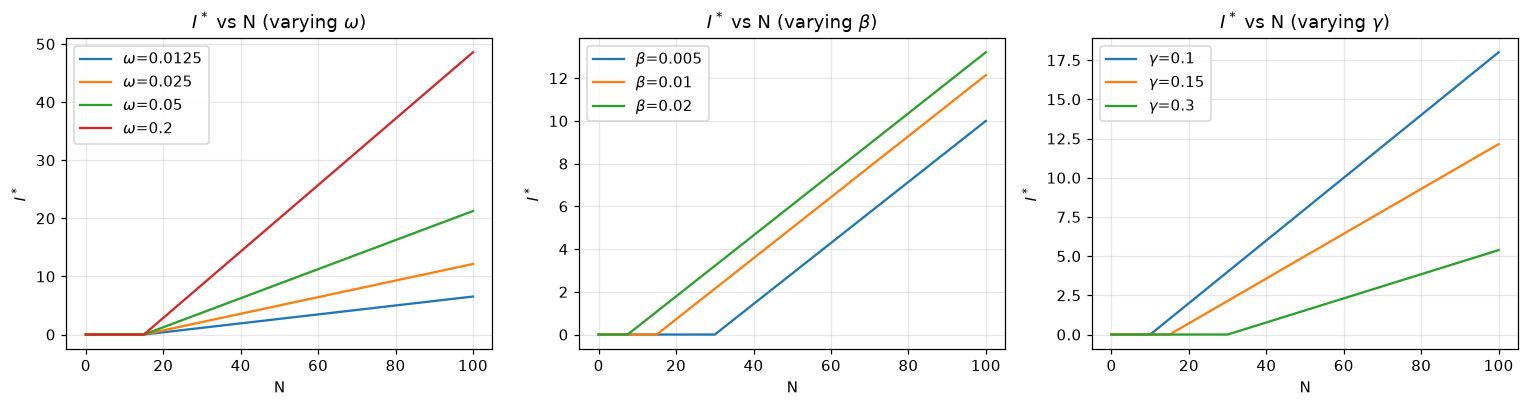
\includegraphics[width=\textwidth]{img/fig2.png}
\begin{itemize}\setlength\itemsep{0.3em}
  \item Grows linearly with $N$. But $S^*=\gamma/\beta$ does not depend on $N$: extra people end up in $I$ and $R$.
  \item Increases with $\beta$ and with $\omega$. If $\omega\to0$ we are back to SIR and $I^*\to0$.
  \item Decreases with $\gamma$ (shorter infections, higher threshold).
\end{itemize}
\end{frame}

% ---------------- Parameters ----------------
\begin{frame}{Q4. Why these parameters?}
\renewcommand{\arraystretch}{1.5}
\centering
\begin{tabular}{l l p{0.5\textwidth}}
\rowcolor{aimsred}\color{white}\bfseries Parameter & \color{white}\bfseries Value & \color{white}\bfseries Meaning\\
$\gamma$ & 0.15 day$^{-1}$ & Infectious period of about 6.7 days\\
\rowcolor{rowpink} $\omega$ & 0.025 day$^{-1}$ & Immunity lasts about 40 days\\
$\beta$ & 0.01 day$^{-1}$ & Puts the threshold $N_c=\gamma/\beta=15$ inside the range $10\le N\le100$\\
\rowcolor{rowpink} $T$ & 365 days & Roughly nine immunity periods, enough for transients to settle\\
\end{tabular}
\vspace{1em}
\callout{0.85\textwidth}{$N=10$ gives $\mathcal R_0=0.67<1$ (no endemic state). \quad $N\ge20$ gives $\mathcal R_0>1$.}
\end{frame}

% ---------------- ODE results ----------------
\begin{frame}{Q4. Numerical ODE solutions}
\centering
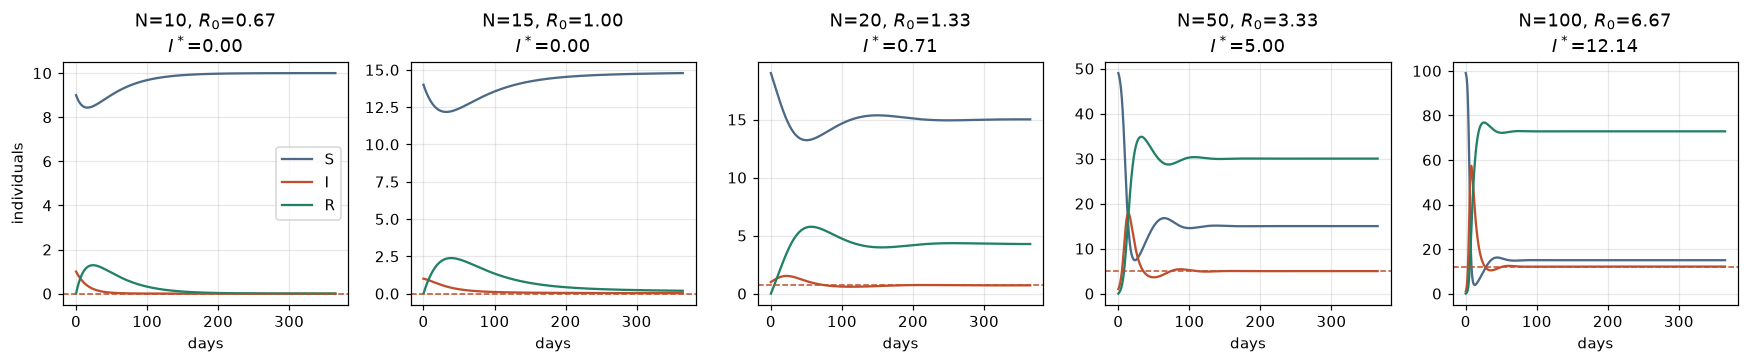
\includegraphics[width=\textwidth]{img/fig3.png}\\[0.3em]
\small
\begin{tabular}{rrrrrr}
\rowcolor{aimsred}\color{white}$N$ & \color{white}10 & \color{white}20 & \color{white}30 & \color{white}50 & \color{white}100\\
$I^*$ theory & 0 & 0.71 & 2.14 & 5.00 & 12.14\\
\rowcolor{rowpink} $I$ from ODE (long run) & 0 & 0.71 & 2.14 & 5.00 & 12.14\\
\end{tabular}
\begin{itemize}
  \item $N=10$: the infection dies out. $N>15$: an epidemic peak, then damped oscillations toward $I^*$.
  \item The numerics match the analysis. Close to $N_c$ the approach is slow.
\end{itemize}
\end{frame}

% ---------------- SSA ----------------
\begin{frame}{Q5. Gillespie SSA with the new event}
\begin{enumerate}\setlength\itemsep{0.6em}
  \item Compute the three propensities: $\beta SI,\ \gamma I,\ \omega R$, and their sum $a_0$.
  \item Draw the waiting time $\tau\sim\mathrm{Exp}(a_0)$.
  \item Pick the event with probability $a_j/a_0$ and update $[S,I,R]$.
  \item Stop at $t=365$ days, or when $I=0$.
\end{enumerate}
\callout{0.85\textwidth}{$I=0$ is an \textbf{absorbing state}: without an infectious person, nobody can be infected again.}
\begin{itemize}
  \item Start: one infectious person, $(S_0,I_0,R_0)=(N-1,1,0)$.
  \item 500 runs for each of 11 values of $N$ between 10 and 100.
\end{itemize}
\end{frame}

% ---------------- Trajectories ----------------
\begin{frame}{Q5. A few SSA runs against the ODE}
\centering
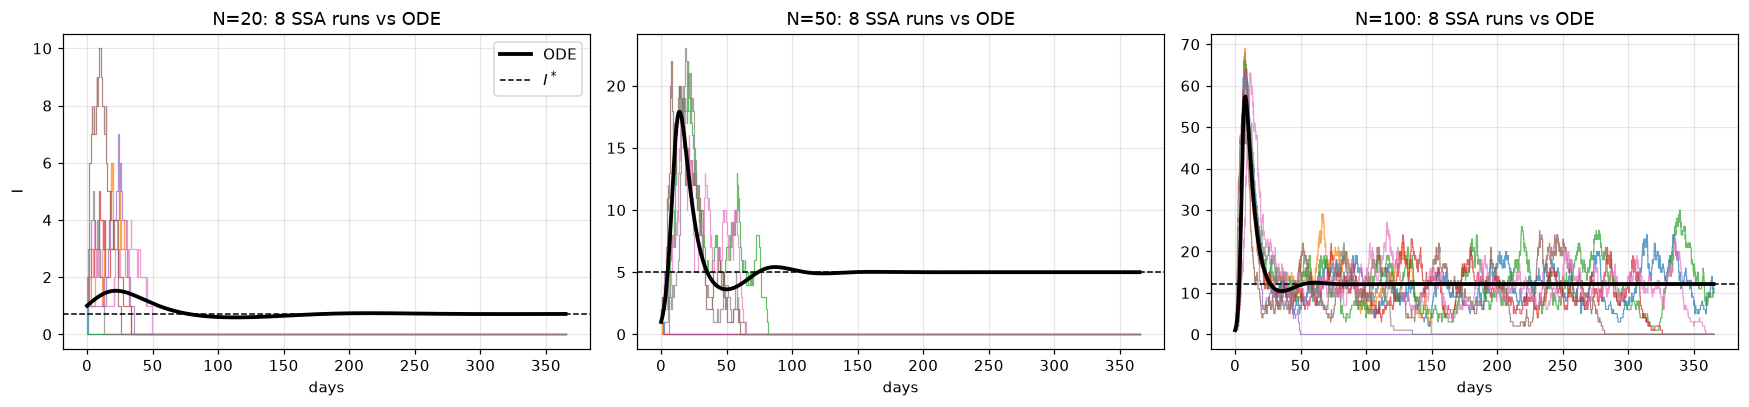
\includegraphics[width=\textwidth]{img/fig4.png}
\begin{itemize}\setlength\itemsep{0.4em}
  \item Black: ODE and its equilibrium $I^*$. Colours: eight stochastic runs.
  \item At $N=20$ and $N=50$ all eight runs here end at $I=0$, while the ODE stays endemic.
  \item At $N=100$ some runs keep fluctuating around the ODE level.
\end{itemize}
\end{frame}

% ---------------- Summary table ----------------
\begin{frame}{Q5. Results over 500 runs}
\small
\renewcommand{\arraystretch}{1.25}
\centering
\begin{tabular}{r r r r r r r r}
\rowcolor{aimsred}\color{white}$N$ & \color{white}$\mathcal R_0$ & \color{white}$I^*$ & \color{white}P(alive) & \color{white}median fade out & \color{white}max $I$ SSA & \color{white}max $I$ ODE & \color{white}mean $I$ alive\\
10 & 0.67 & 0 & 0.00 & 5.5 d & 1.67 & 1.00 & n/a\\
\rowcolor{rowpink} 15 & 1.00 & 0 & 0.00 & 5.9 d & 2.01 & 1.00 & n/a\\
20 & 1.33 & 0.71 & 0.00 & 6.1 d & 2.83 & 1.52 & n/a\\
\rowcolor{rowpink} 25 & 1.67 & 1.43 & 0.00 & 10.1 d & 4.11 & 3.22 & n/a\\
30 & 2.00 & 2.14 & 0.00 & 11.5 d & 5.32 & 5.54 & n/a\\
\rowcolor{rowpink} 40 & 2.67 & 3.57 & 0.00 & 42.2 d & 10.45 & 11.26 & n/a\\
50 & 3.33 & 5.00 & 0.00 & 48.1 d & 14.73 & 17.90 & 5.12\\
\rowcolor{rowpink} 70 & 4.67 & 7.86 & 0.07 & 64.5 d & 27.24 & 32.80 & 8.00\\
100 & 6.67 & 12.14 & 0.56 & 99.7 d & 52.57 & 57.37 & 11.99\\
\end{tabular}
\\[0.6em]
{\footnotesize P(alive) is the fraction of runs with $I>0$ at day 365. Mean $I$ is averaged over days 100 to 365 for surviving runs.}
\end{frame}

% ---------------- Summary plots ----------------
\begin{frame}{Q5. Persistence, peak and mean level versus $N$}
\centering
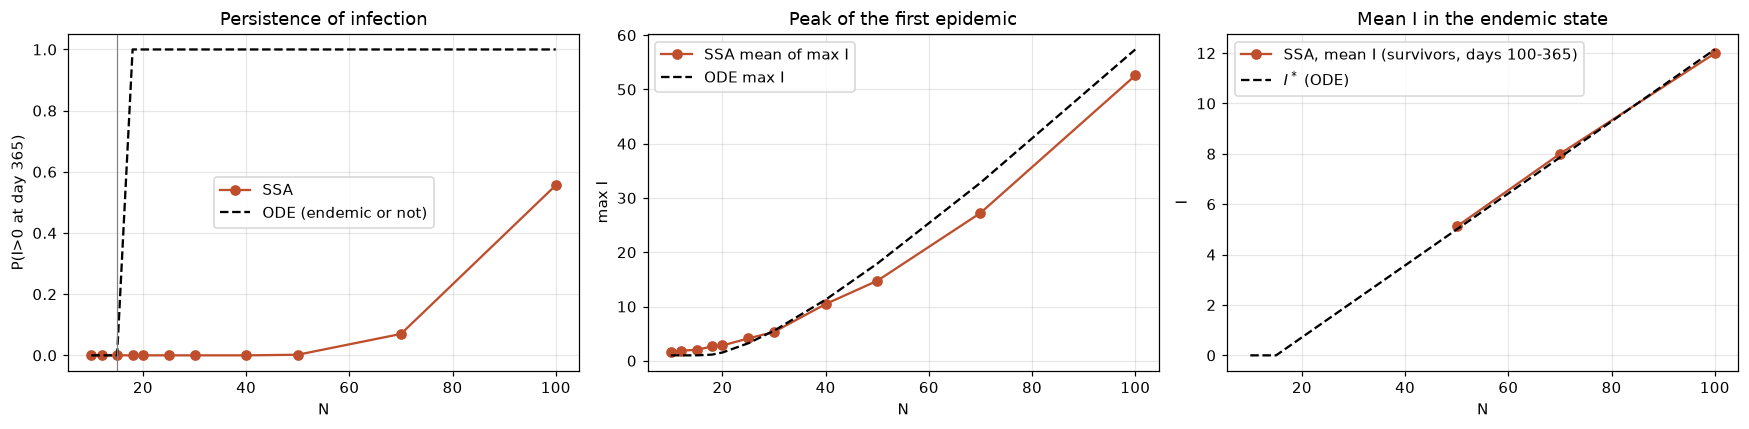
\includegraphics[width=\textwidth]{img/fig5.png}
\begin{itemize}\setlength\itemsep{0.4em}
  \item \hl{Persistence:} the ODE predicts an endemic state for all $N>15$. In the SSA no run survived up to $N=40$, 1 of 500 at $N=50$, 35 of 500 (7\%) at $N=70$ and 278 of 500 (56\%) at $N=100$.
  \item \hl{Peak:} higher in the SSA for small $N$, lower for large $N$ (some runs die before taking off).
  \item \hl{Mean level:} when the infection survives, its mean is close to $I^*$.
\end{itemize}
\end{frame}

% ---------------- Fade out ----------------
\begin{frame}{Q5. Where does the infection end up, and when does it vanish?}
\centering
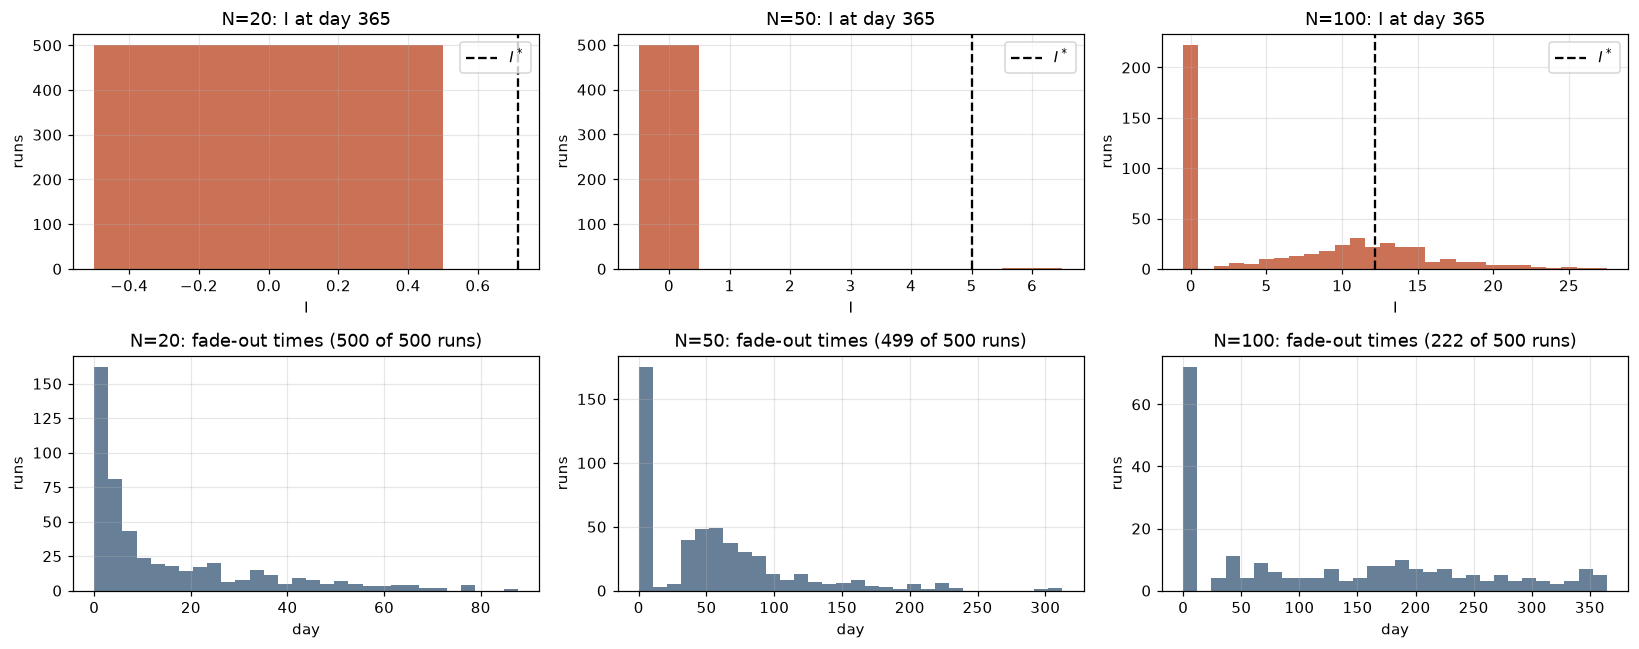
\includegraphics[width=0.95\textwidth]{img/fig6.png}
\begin{itemize}\setlength\itemsep{0.4em}
  \item At $N=100$ the day 365 distribution has a mass at zero and a second group near $I^*\approx12$.
  \item Fade out gets later as $N$ grows: median about 10 days at $N=25$, 48 days at $N=50$, 100 days at $N=100$.
\end{itemize}
\end{frame}

% ---------------- Answers ----------------
\begin{frame}{Q5. Answers to the guiding questions}
\begin{itemize}\setlength\itemsep{0.7em}
  \item \hl{Does the SSA always give an endemic state when the ODE does?} No. For $N$ from 18 to 40, zero out of 500 runs were still infected at day 365, and only 1 of 500 at $N=50$.
  \item \hl{How often do they differ?} For all $N>15$ up to 100, at least partly. They only fully agree for $N\le15$.
  \item \hl{Maximum of $I$?} The SSA peak is above the ODE peak for small $N$ and below it for large $N$.
  \item \hl{Mean $I$ in the endemic state?} Close to $I^*$: 5.1 vs 5.0 at $N=50$, 8.0 vs 7.9 at $N=70$, 12.0 vs 12.1 at $N=100$.
\end{itemize}
\callout{0.9\textwidth}{For $N=18$ to $25$, $I^*$ is below one person. A fraction of a person cannot persist, so $N>N_c$ is necessary but not sufficient for persistence in a small population.}
\end{frame}

% ---------------- Conclusion ----------------
\begin{frame}{Take home message}
\begin{itemize}\setlength\itemsep{0.9em}
  \item With waning immunity, the ODE predicts an endemic equilibrium when $N>\gamma/\beta$, with $I^*=\frac{\omega}{\omega+\gamma}\big(N-\frac{\gamma}{\beta}\big)$.
  \item The ODE is the large population picture. It never lets $I$ reach exactly zero.
  \item In small populations chance matters. The SSA adds a new outcome, \hl{stochastic extinction}, even when $\mathcal R_0>1$.
  \item When the infection does persist, its average level agrees with the ODE.
\end{itemize}
\callout{0.8\textwidth}{Next: Part 2, two strains with waning immunity and cross infection.}
\end{frame}

% =====================================================================
%                              PART 2
% =====================================================================
\begin{frame}[plain]
\centering\vspace{5em}
{\Large\bfseries\color{aimsred} Part 2\\[0.5em] Two strains with waning immunity}\\[1.2em]
{\large\color{textgrey} ODE versus Gillespie SSA, population size $N=10{,}000$, 50 years}
\end{frame}

\begin{frame}{The model and three points to settle}
\begin{itemize}\setlength\itemsep{0.5em}
  \item Five classes: $S$, $I_1$, $I_2$, $R_1$, $R_2$. Births into $S$ and deaths at rate $\mu$ from every class.
  \item Waning immunity sends $R_i$ back to $S$. Someone recovered from one strain can still catch the other.
\end{itemize}
\vspace{0.3em}
\begin{enumerate}\setlength\itemsep{0.6em}
  \item The sheet says ``$\beta_1$ and $\beta_1$''. It must be $\beta_1$ and $\beta_2$.
  \item Equations (2.2) to (2.5) leave out the cross infections $\beta_1R_2I_1$ and $\beta_2R_1I_2$, but the text, the code and the 14 SSA events include them. We use the \textbf{full model} and also run the printed equations for comparison.
  \item Here the ODE is in proportions, so the SSA infection propensity is $\beta SI/N$. (In Part 1 we worked with counts, so it was $\beta SI$. It is the same model with $\beta_{\rm counts}=\beta/N$.)
\end{enumerate}
\end{frame}

\begin{frame}{Investigation 1. Cartoon network}
\centering
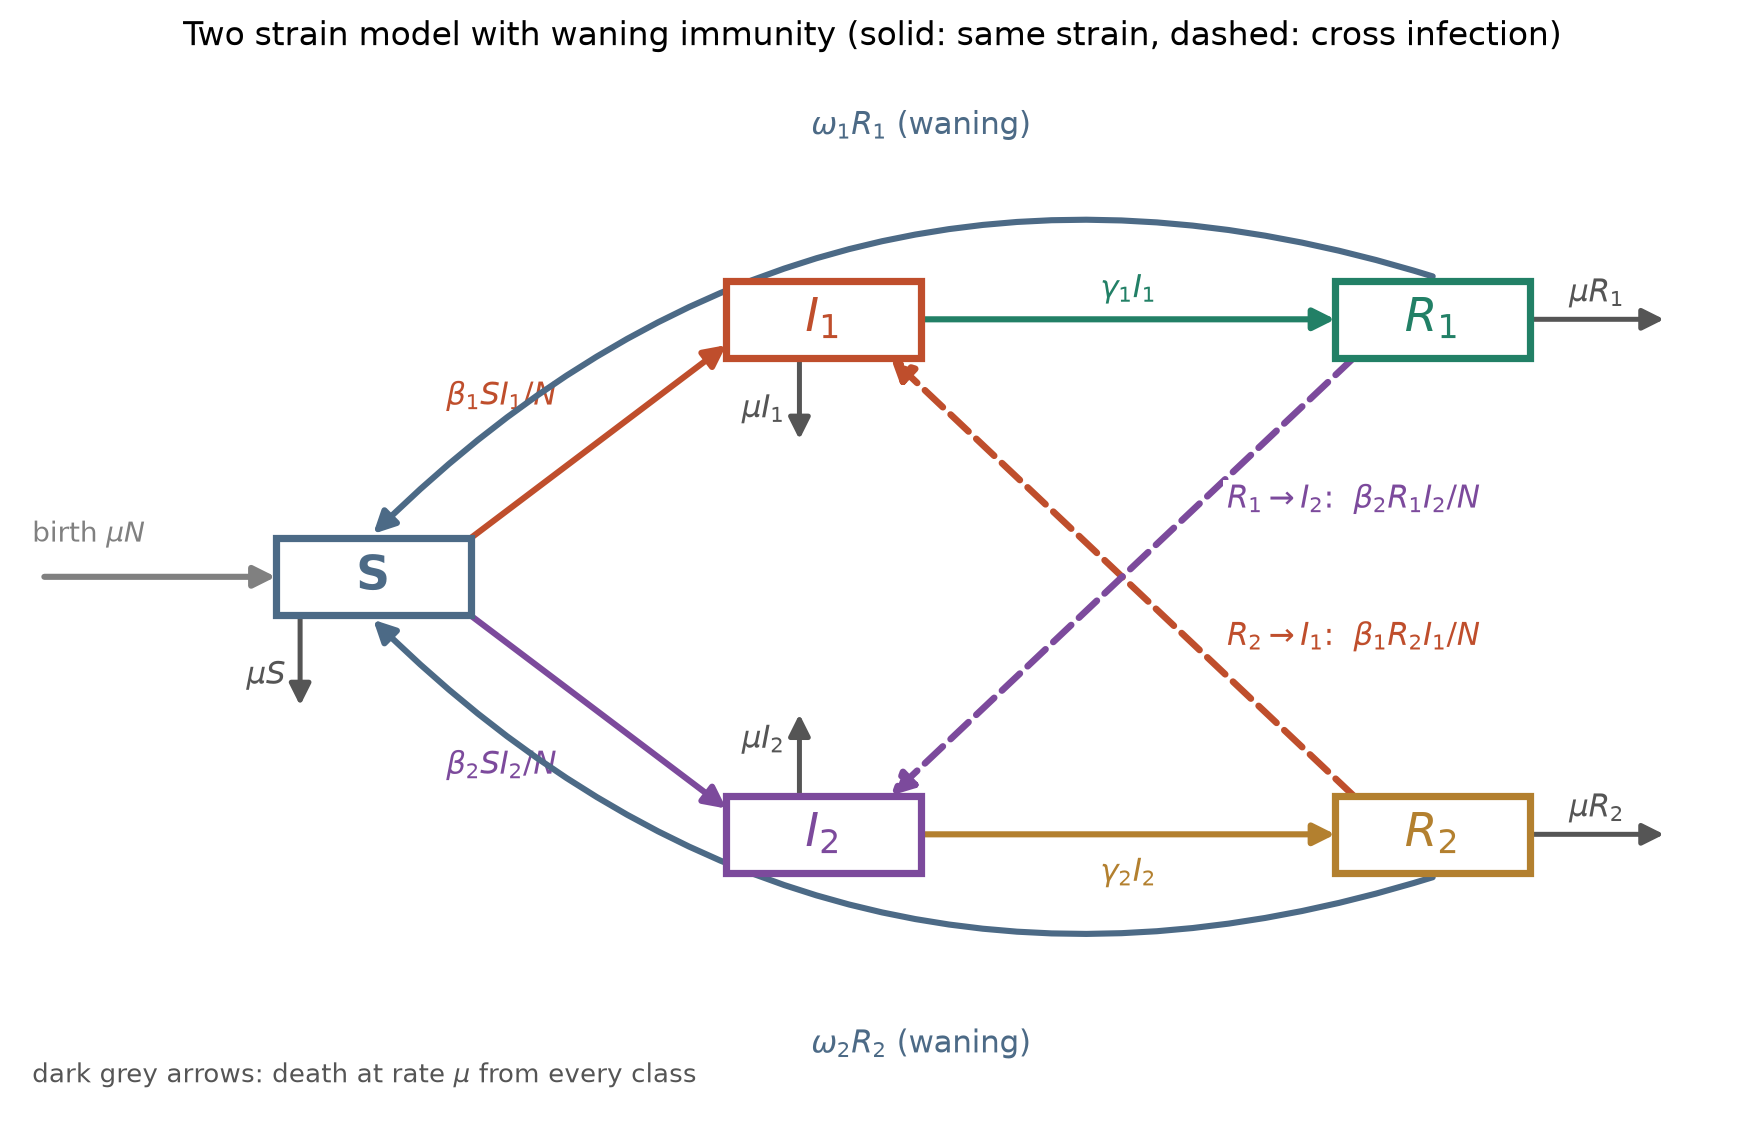
\includegraphics[width=0.82\textwidth]{img/p2fig1.png}
\end{frame}

\begin{frame}{The 14 events (state $[S,I_1,I_2,R_1,R_2]$)}
\small
\renewcommand{\arraystretch}{1.18}
\centering
\begin{tabular}{r l l l}
\rowcolor{aimsred}\color{white}\# & \color{white}Event & \color{white}Change & \color{white}Propensity\\
0 & Birth into $S$ & $[+1,0,0,0,0]$ & $\mu N$\\
\rowcolor{rowpink} 1 to 5 & Death of $S,I_1,I_2,R_1,R_2$ & $-1$ in that class & $\mu S,\mu I_1,\mu I_2,\mu R_1,\mu R_2$\\
6 & $S\to I_1$ & $[-1,+1,0,0,0]$ & $\beta_1SI_1/N$\\
\rowcolor{rowpink} 7 & $S\to I_2$ & $[-1,0,+1,0,0]$ & $\beta_2SI_2/N$\\
8 & $R_2\to I_1$ & $[0,+1,0,0,-1]$ & $\beta_1R_2I_1/N$\\
\rowcolor{rowpink} 9 & $R_1\to I_2$ & $[0,0,+1,-1,0]$ & $\beta_2R_1I_2/N$\\
10 & $I_1\to R_1$ & $[0,-1,0,+1,0]$ & $\gamma_1I_1$\\
\rowcolor{rowpink} 11 & $I_2\to R_2$ & $[0,0,-1,0,+1]$ & $\gamma_2I_2$\\
12 & $R_1\to S$ (waning) & $[+1,0,0,-1,0]$ & $\omega_1R_1$\\
\rowcolor{rowpink} 13 & $R_2\to S$ (waning) & $[+1,0,0,0,-1]$ & $\omega_2R_2$\\
\end{tabular}
\\[0.6em]
{\footnotesize These are the propensities the sheet asks us to complete.}
\end{frame}

\begin{frame}{Investigation 2. Eliminating one variable}
\small
Adding the five equations: $\dfrac{d}{dt}(S+I_1+I_2+R_1+R_2)=\mu\,(1-\text{total})$, so the total stays at 1.\\[0.4em]
Put $S=1-I_1-I_2-R_1-R_2$. The equation for $S$ is redundant and the others become
\[
\begin{aligned}
\dot I_1&=\beta_1(1-I_1-I_2-R_1)I_1-(\gamma_1+\mu)I_1\\
\dot I_2&=\beta_2(1-I_1-I_2-R_2)I_2-(\gamma_2+\mu)I_2\\
\dot R_1&=\gamma_1I_1-\beta_2R_1I_2-(\omega_1+\mu)R_1\\
\dot R_2&=\gamma_2I_2-\beta_1R_2I_1-(\omega_2+\mu)R_2
\end{aligned}
\]
\begin{itemize}\setlength\itemsep{0.3em}
  \item In $\dot I_1$ the cross term $+\beta_1R_2I_1$ cancels the $-R_2$ that comes from $S$. The people susceptible to strain 1 are $S+R_2=1-I_1-I_2-R_1$.
  \item We checked the algebra symbolically (sympy): the difference is zero.
\end{itemize}
\end{frame}

\begin{frame}{Investigation 3. Parameters and basic reproduction numbers}
\renewcommand{\arraystretch}{1.4}
\centering
\begin{tabular}{l c c c c}
\rowcolor{aimsred}\color{white}& \color{white}$\beta$ & \color{white}$\gamma$ & \color{white}$\omega$ & \color{white}$\mathcal R_0=\beta/(\gamma+\mu)$\\
Strain 1 & 120 & 52 (1 week) & 0.2 (5 years) & $\mathbf{2.31}$\\
\rowcolor{rowpink} Strain 2 & 100 & 26 (2 weeks) & 0.5 (2 years) & $\mathbf{3.84}$\\
\end{tabular}
\\[0.8em]
All rates per year. $\mu=0.02$ per year, $N=10{,}000$, initial state $[9900,50,50,0,0]$.
\callout{0.85\textwidth}{Both $\mathcal R_0>1$, and strain 2 has the larger one. Classical theory would let strain 2 win.}
\begin{itemize}
  \item The sheet's SSA function stores every event: about 220,000 per simulated year, so about 6 seconds per year. We checked it on a short run, and used a faster version of the same algorithm for 50 years.
\end{itemize}
\end{frame}

\begin{frame}{Investigation 3. ODE and SSA side by side}
\centering
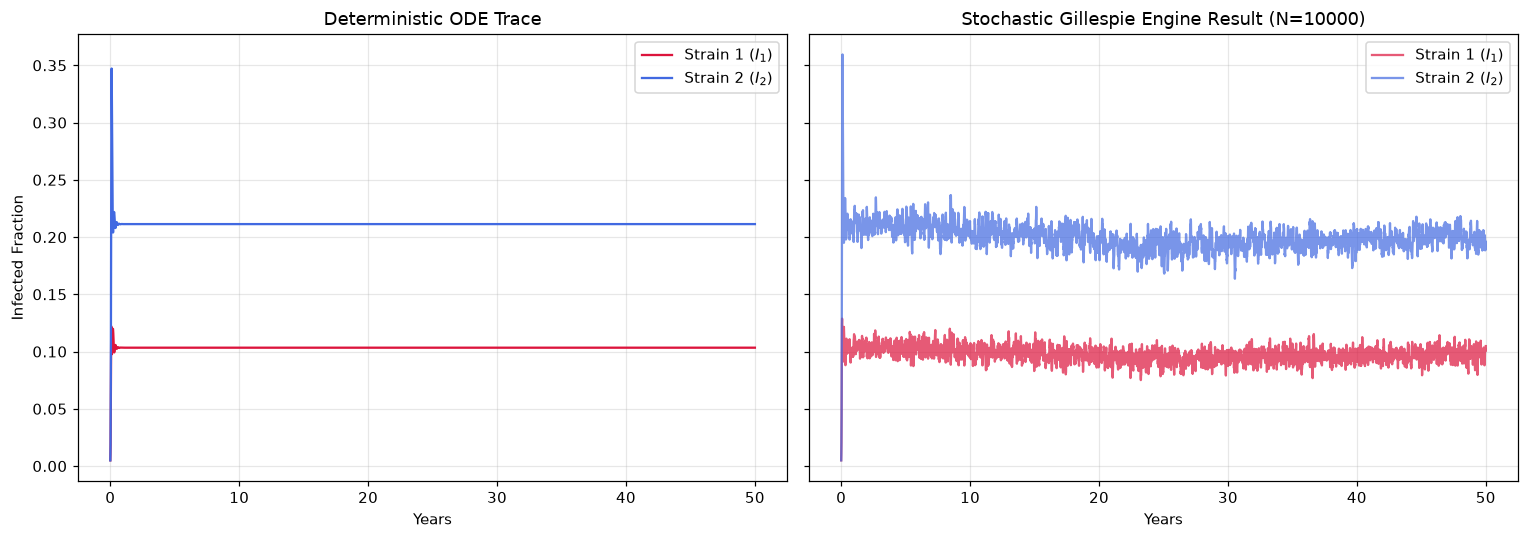
\includegraphics[width=\textwidth]{img/p2fig2.png}
\begin{itemize}\setlength\itemsep{0.3em}
  \item Both strains settle quickly. The SSA fluctuates around the ODE levels (standard deviation about 0.006 and 0.009).
  \item ODE: $I_1^*=0.103$, $I_2^*=0.211$. SSA means over years 10 to 50: 0.096 and 0.197 in this run.
\end{itemize}
\end{frame}

\begin{frame}{Why the SSA level differs a little from the ODE}
\small
\centering
\begin{tabular}{l r r r}
\rowcolor{aimsred}\color{white}Run (20 years) & \color{white}mean total & \color{white}mean $I_1/N$ & \color{white}mean $I_2/N$\\
1 & 10,043 & 0.1046 & 0.2137\\
\rowcolor{rowpink} 2 & 9,905 & 0.0997 & 0.2047\\
3 & 9,966 & 0.1022 & 0.2092\\
\rowcolor{rowpink} 4 & 9,999 & 0.1034 & 0.2114\\
ODE & 10,000 & 0.1034 & 0.2113\\
\end{tabular}
\vspace{0.8em}
\begin{itemize}\setlength\itemsep{0.5em}
  \item In the sheet's SSA, births and deaths are separate random events, so the total population is not fixed. In the 50 year run it ranged from 9,686 to 10,031.
  \item The mean infected level changes by a few percent from run to run (strain 1: 0.096 to 0.105 over five runs, against 0.103). The ODE conserves the total exactly.
  \item The sheet's own SSA code, the fast version and the ODE agree on the mean state after half a year (for example $I_1$: 100.8, 102.5 and 102.4 people at $N=1000$).
\end{itemize}
\end{frame}

\begin{frame}{Investigation 4. Steady coexistence, not cycles}
\begin{columns}[T]
\column{0.52\textwidth}
\begin{itemize}\setlength\itemsep{0.5em}
  \item Overshoot in the first month (peaks near 0.12 and 0.35), then a damped oscillation.
  \item Jacobian eigenvalues: $-8.25\pm33.1i$, $-32.6$, $-18.8$. All negative real parts, so the equilibrium is stable.
  \item Period of the transient about 69 days, half life about one month. No sustained cycles.
\end{itemize}
\column{0.45\textwidth}
\renewcommand{\arraystretch}{1.3}
\begin{tabular}{l r}
\rowcolor{aimsred}\color{white}Class & \color{white}Equilibrium\\
$S^*$ & 0.0084\\
\rowcolor{rowpink} $I_1^*$ & 0.1034\\
$I_2^*$ & 0.2113\\
\rowcolor{rowpink} $R_1^*$ & 0.2518\\
$R_2^*$ & 0.4251\\
\end{tabular}
\end{columns}
\vspace{0.6em}
\callout{0.9\textwidth}{Checked: $S^*+R_2^*=1/\mathcal R_0^1=0.4335$ and $S^*+R_1^*=1/\mathcal R_0^2=0.2602$.}
\end{frame}

\begin{frame}{Why can both strains coexist?}
Strain $i$ alone settles at $S=1/\mathcal R_0^i$. A rare newcomer $j$ faces $S+R_i=1-I_i^*$ susceptible people, so
\[ \mathcal R_{\rm inv}^{\,j\ \mathrm{into}\ i}=\mathcal R_0^{\,j}\,(1-I_i^*). \]
\renewcommand{\arraystretch}{1.35}
\centering
\begin{tabular}{l c c}
\rowcolor{aimsred}\color{white}& \color{white}Strain alone, $I^*$ & \color{white}Invasion number\\
Strain 2 invading strain 1 & $I_1^*=0.0024$ & $3.83>1$\\
\rowcolor{rowpink} Strain 1 invading strain 2 & $I_2^*=0.0145$ & $2.27>1$\\
\end{tabular}
\begin{itemize}\setlength\itemsep{0.4em}
  \item Each strain can invade the other, so neither is excluded.
  \item People recovered from one strain are fresh hosts for the other.
  \item Together they carry far more infection than alone: 43 times more for strain 1 and 15 times more for strain 2.
\end{itemize}
\end{frame}

\begin{frame}{The equations as printed give competitive exclusion}
\centering
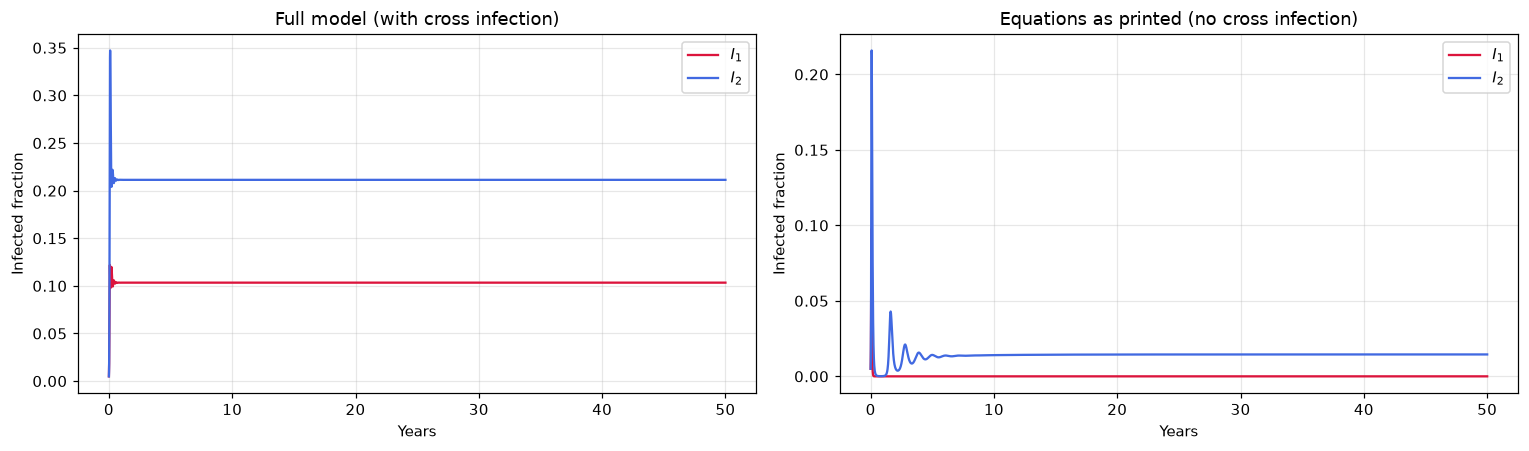
\includegraphics[width=0.95\textwidth]{img/p2fig4.png}
\begin{itemize}\setlength\itemsep{0.3em}
  \item Without cross infection, strain 2 (larger $\mathcal R_0$) wins. At year 50: $I_1\approx10^{-40}$ and $I_2=0.0145$.
  \item So the cross infection is what turns exclusion into coexistence.
\end{itemize}
\end{frame}

\begin{frame}{Stochastic extinction versus deterministic permanence}
\centering
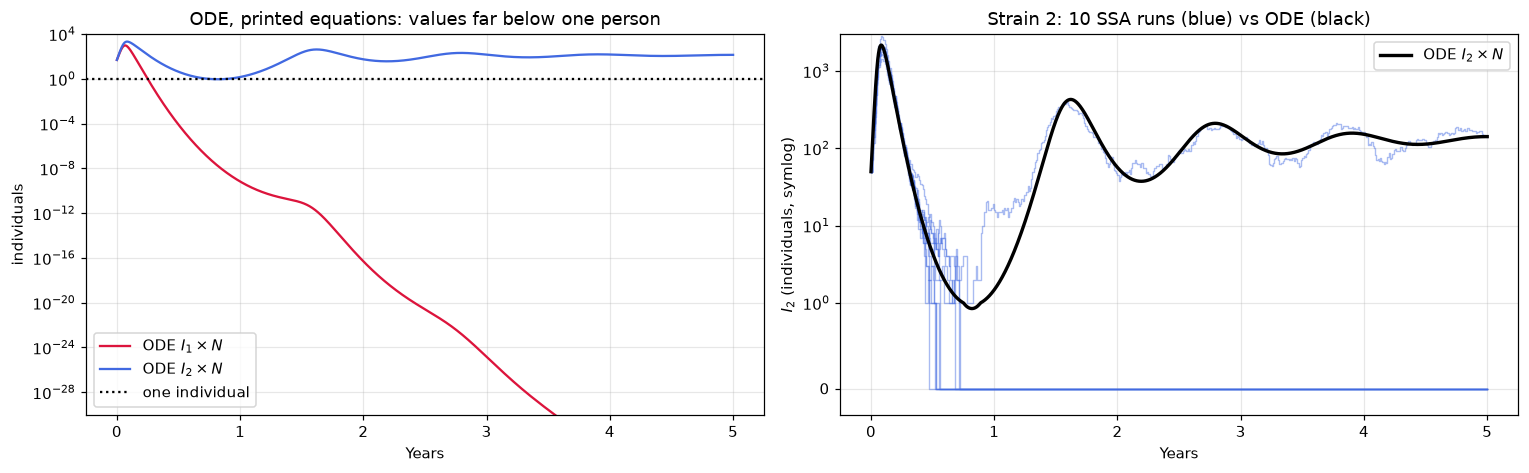
\includegraphics[width=0.95\textwidth]{img/p2fig5.png}
\begin{itemize}\setlength\itemsep{0.3em}
  \item Printed equations. ODE: strain 2 peaks, then dips to 0.93 individuals (year 0.82) and rebounds to 142 individuals by year 5.
  \item SSA, 40 runs: strain 1 lost in 100\% of runs and strain 2 in 85\%. Zero is absorbing, so a lost strain never rebounds.
\end{itemize}
\end{frame}

\begin{frame}{What happens at zero, and why it matters}
\begin{itemize}\setlength\itemsep{0.8em}
  \item \hl{In the SSA:} when $I_i=0$, the infection events of strain $i$ have propensity zero and nothing else creates infection (no immigration). The strain is gone for good.
  \item \hl{In the ODE:} $I_i$ can be tiny and positive and recover later. A fraction $10^{-4}$ of 10,000 people is about one person. $10^{-14}$ is $10^{-10}$ of a person.
  \item \hl{Effect on competition:} a temporary dip in the ODE becomes a permanent loss in the SSA. The survivor is decided by chance as well as by $\mathcal R_0$.
  \item \hl{In the full model at $N=10{,}000$:} no extinction in 50 years, and no crash after the first peak. The ``tiny value then rebound'' picture of the sheet appears for strain 2 in the printed equations, not in the full model.
\end{itemize}
\end{frame}

\begin{frame}{Full model at smaller $N$: extinction appears}
\small
\renewcommand{\arraystretch}{1.3}
\centering
\begin{tabular}{r c c c c c}
\rowcolor{aimsred}\color{white}$N$ & \color{white}start per strain & \color{white}ODE $I_1^*,I_2^*$ (people) & \color{white}P(extinct by yr 50) & \color{white}in year 1 & \color{white}after year 1\\
100 & 1 & 10, 21 & 1.00 & 1.00 & 0.00\\
\rowcolor{rowpink} 200 & 1 & 21, 42 & 1.00 & 0.70 & 0.30\\
400 & 2 & 41, 85 & 0.60 & 0.30 & 0.30\\
\rowcolor{rowpink} 700 & 4 & 72, 148 & 0.08 & 0.08 & 0.00\\
1000 & 5 & 103, 211 & 0.02 & 0.02 & 0.00\\
\end{tabular}
\\[0.4em]
{\footnotesize 40 runs per $N$. Strain 1 and strain 2 have the same extinction fraction in every row: they are lost together.}\\[0.4em]
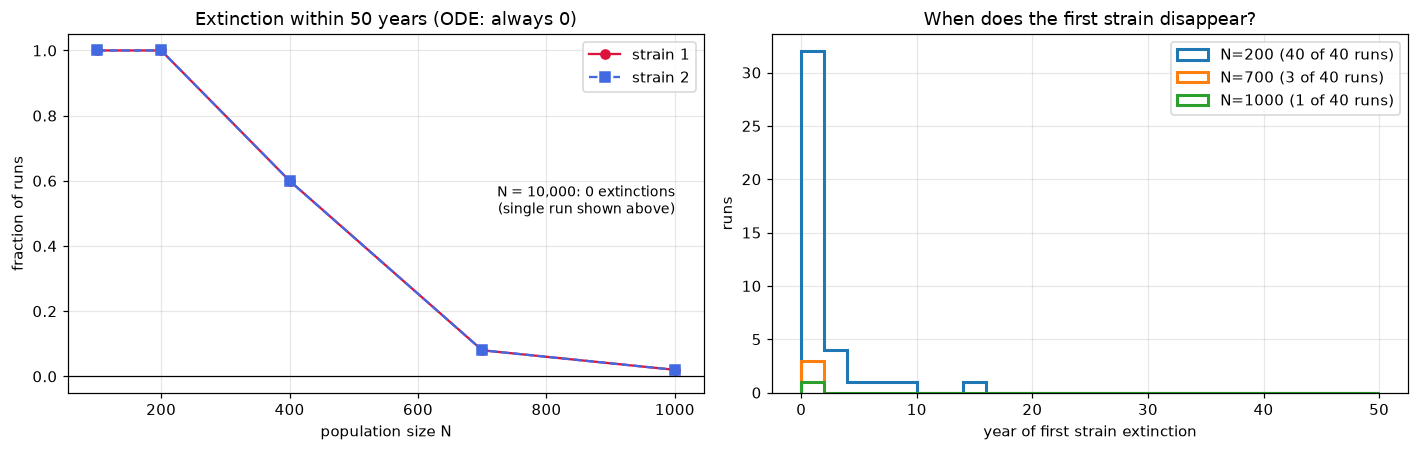
\includegraphics[width=0.78\textwidth]{img/p2fig6.png}
\end{frame}

\begin{frame}{Why the two strains are lost together}
\begin{itemize}\setlength\itemsep{0.8em}
  \item The two strains have the same extinction fraction in every row, and in the example run below they vanish within a quarter of a year of each other.\item Alone, each strain sustains a far smaller infected fraction (0.0024 and 0.0145) than together (0.103 and 0.211).
  \item A likely reason: when one strain disappears, the other is left with very few carriers (for strain 2, about 4 people at $N=300$), and it soon follows. We did not test this mechanism separately.
  \item Coexistence supports itself, and so does collapse.
  \item For $N\ge700$ all extinctions happen in the first year, when only 4 or 5 people carry each strain. For $N\le400$ they also happen later.
\end{itemize}
\centering
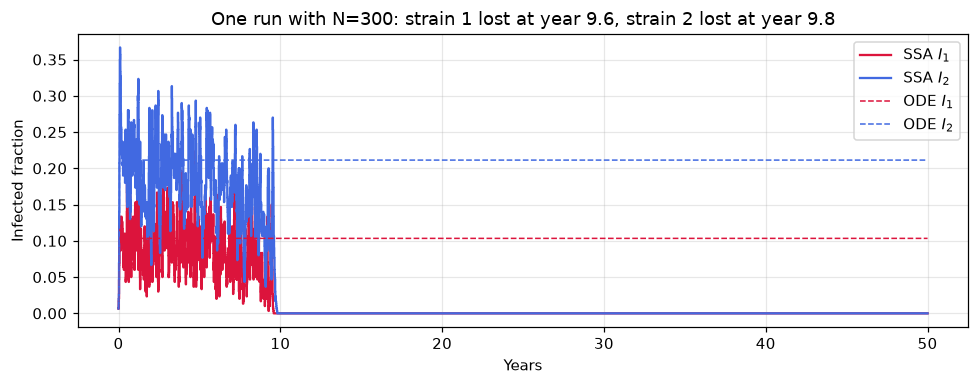
\includegraphics[width=0.62\textwidth]{img/p2fig7.png}
\end{frame}

\begin{frame}{Part 2. Take home message}
\begin{itemize}\setlength\itemsep{0.8em}
  \item With waning immunity and cross infection the ODE gives a \hl{stable coexistence} of both strains, $\mathcal R_0^1=2.31$ and $\mathcal R_0^2=3.84$. No sustained oscillations at these parameters.
  \item Without cross infection (equations as printed) we get classical competitive exclusion.
  \item At $N=10{,}000$ the SSA agrees with the ODE, with fluctuations and a few percent of run to run variation.
  \item At small $N$, or when a strain goes through a bottleneck, the SSA turns tiny ODE values into real extinctions, and extinct strains do not return.
\end{itemize}
\callout{0.9\textwidth}{Deterministic models describe the large population limit. Stochastic models tell us whether a strain actually survives.}
\end{frame}


\end{document}
